\documentclass{beamer}
%
% Choose how your presentation looks.
%
% For more themes, color themes and font themes, see:
% http://deic.uab.es/~iblanes/beamer_gallery/index_by_theme.html
%
\mode<presentation>
{
  \usetheme{Frankfurt}    % or try Darmstadt, Madrid, Warsaw, ...
  \usecolortheme{crane}   % or try albatross, beaver, crane, ...
  \usefonttheme{default}  % or try serif, structurebold, ...
  %\setbeamertemplate{navigation symbols}{}
  \setbeamertemplate{caption}[numbered]
} 

\usepackage[english]{babel}
\usepackage[utf8x]{inputenc}
\usepackage{wrapfig}

\usepackage[]{algorithm2e}

\usepackage{graphicx,calc}
\newlength\myheight
\newlength\mydepth
\settototalheight\myheight{Xygp}
\settodepth\mydepth{Xygp}
\setlength\fboxsep{0pt}
\newcommand*\inlinegraphics[1]{%
  \settototalheight\myheight{Xygp}%
  \settodepth\mydepth{Xygp}%
  \raisebox{-\mydepth}{\includegraphics[height=\myheight]{#1}}%
}


\title[Your Short Title]{Greedy Heuristics for set cover}
\author{Eirini Asteri, Jessica Hoffmann}
\institute{University of Texas, Austin}
\date{}

\begin{document}

\begin{frame}
  \titlepage
\end{frame}

% Uncomment these lines for an automatically generated outline.
\begin{frame}{Outline}
  \tableofcontents
\end{frame}

\begin{frame}
\frametitle{Set Cover Problem \& Greedy Algorithm}
\begin{minipage}{0.45\textwidth}
\begin{overlayarea}{\textwidth}{0.5\textheight}
\only<1>{
\includegraphics[width=\columnwidth]{frame1.pdf}}% 
\only<2>{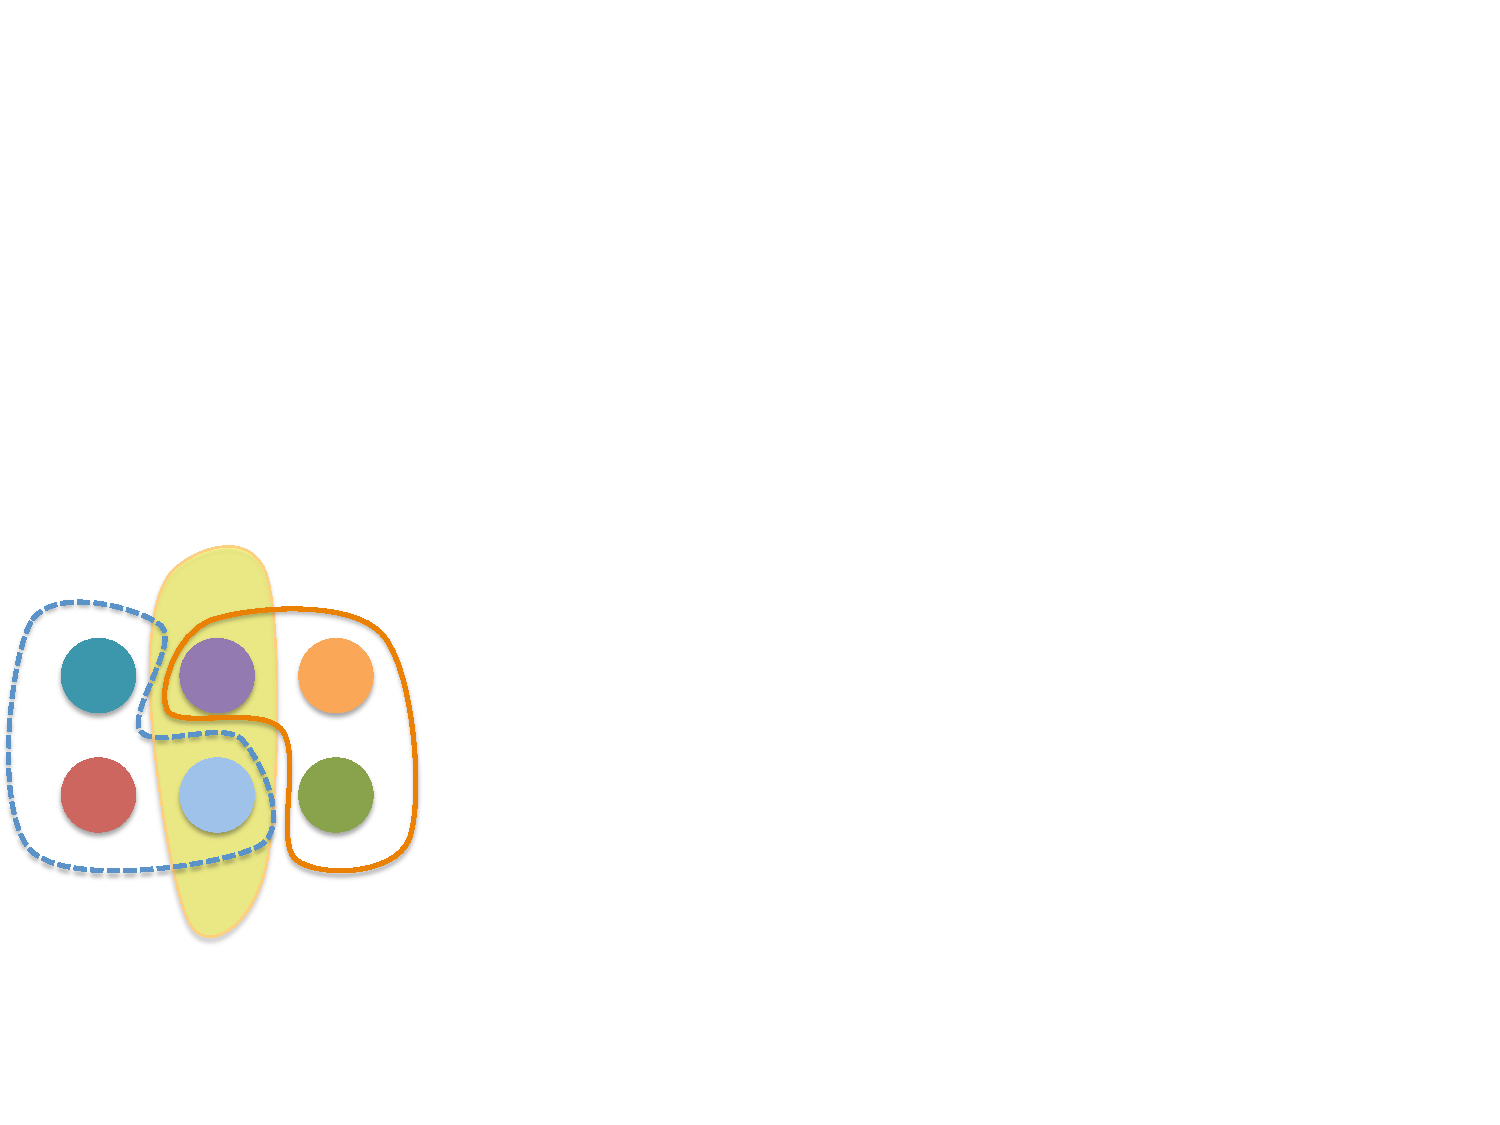
\includegraphics[width=\columnwidth]{frame2.pdf}}% 
\only<3-5>{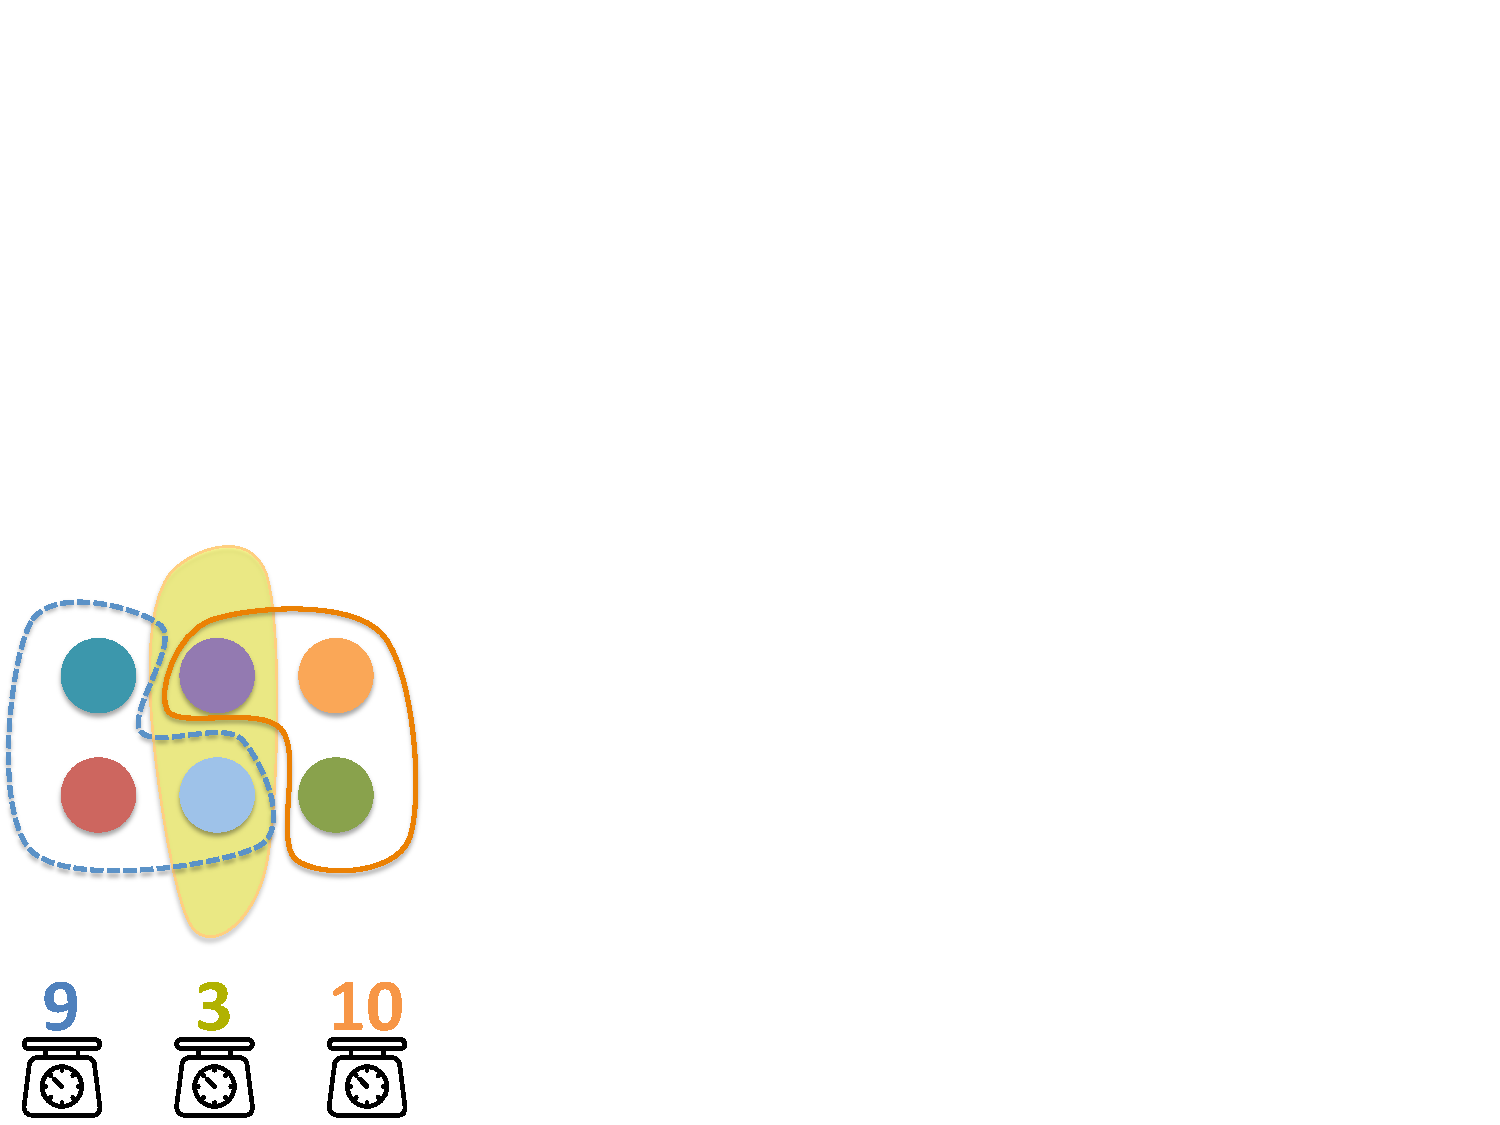
\includegraphics[width=\columnwidth]{frame3.pdf}}%
\end{overlayarea}%
\end{minipage}%
\begin{minipage}{0.55\textwidth} 
\begin{itemize}
\item<1-> Number of distinct elements $e_i$
\item<2-> Number of sets $S_j$
\item<3-> A weight for each set $w_j$
\item<4-> \textbf{Goal} Find set cover with minimum weight
\item<5> \textbf{Greedy Choice} $$best\_set = \arg \min_{l} \cfrac{w_l}{\hat{S}_l}$$
\end{itemize}
\end{minipage}
\end{frame}

\begin{frame}
\frametitle{Basic Preprocessing}
\begin{block}{Get rid of redundant sets \inlinegraphics{sweep.eps}}
If $S_{small} \subseteq S_{big}$ and $\text{weight}(S_{small})\geq \text{weight}(S_{big})$ then $S_{small}$ is a redundant set.
\end{block}
\end{frame}

\begin{frame}
\frametitle{Theoretical Analysis}
\end{frame}

\begin{frame}
\frametitle{Heuristics [Intuition]}
\begin{minipage}{0.30\textwidth}
\begin{overlayarea}{\textwidth}{0.5\textheight}
\only<1-3>{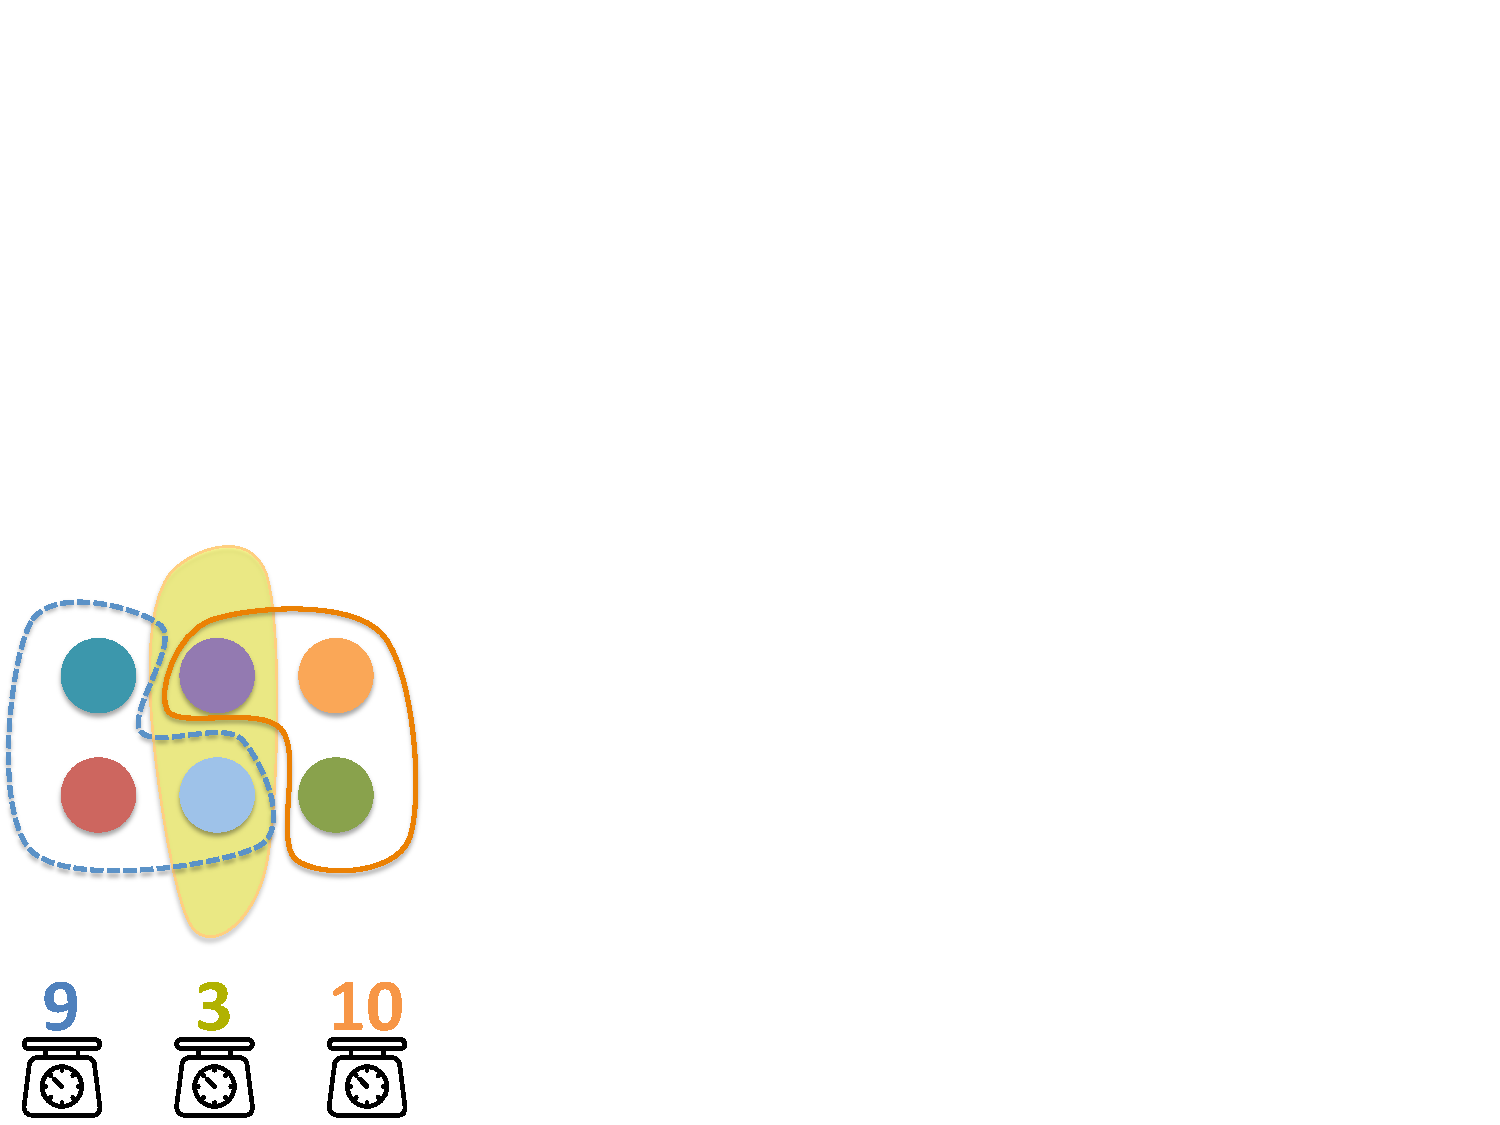
\includegraphics[width=\columnwidth]{frame3.pdf}}% 
\only<4-5>{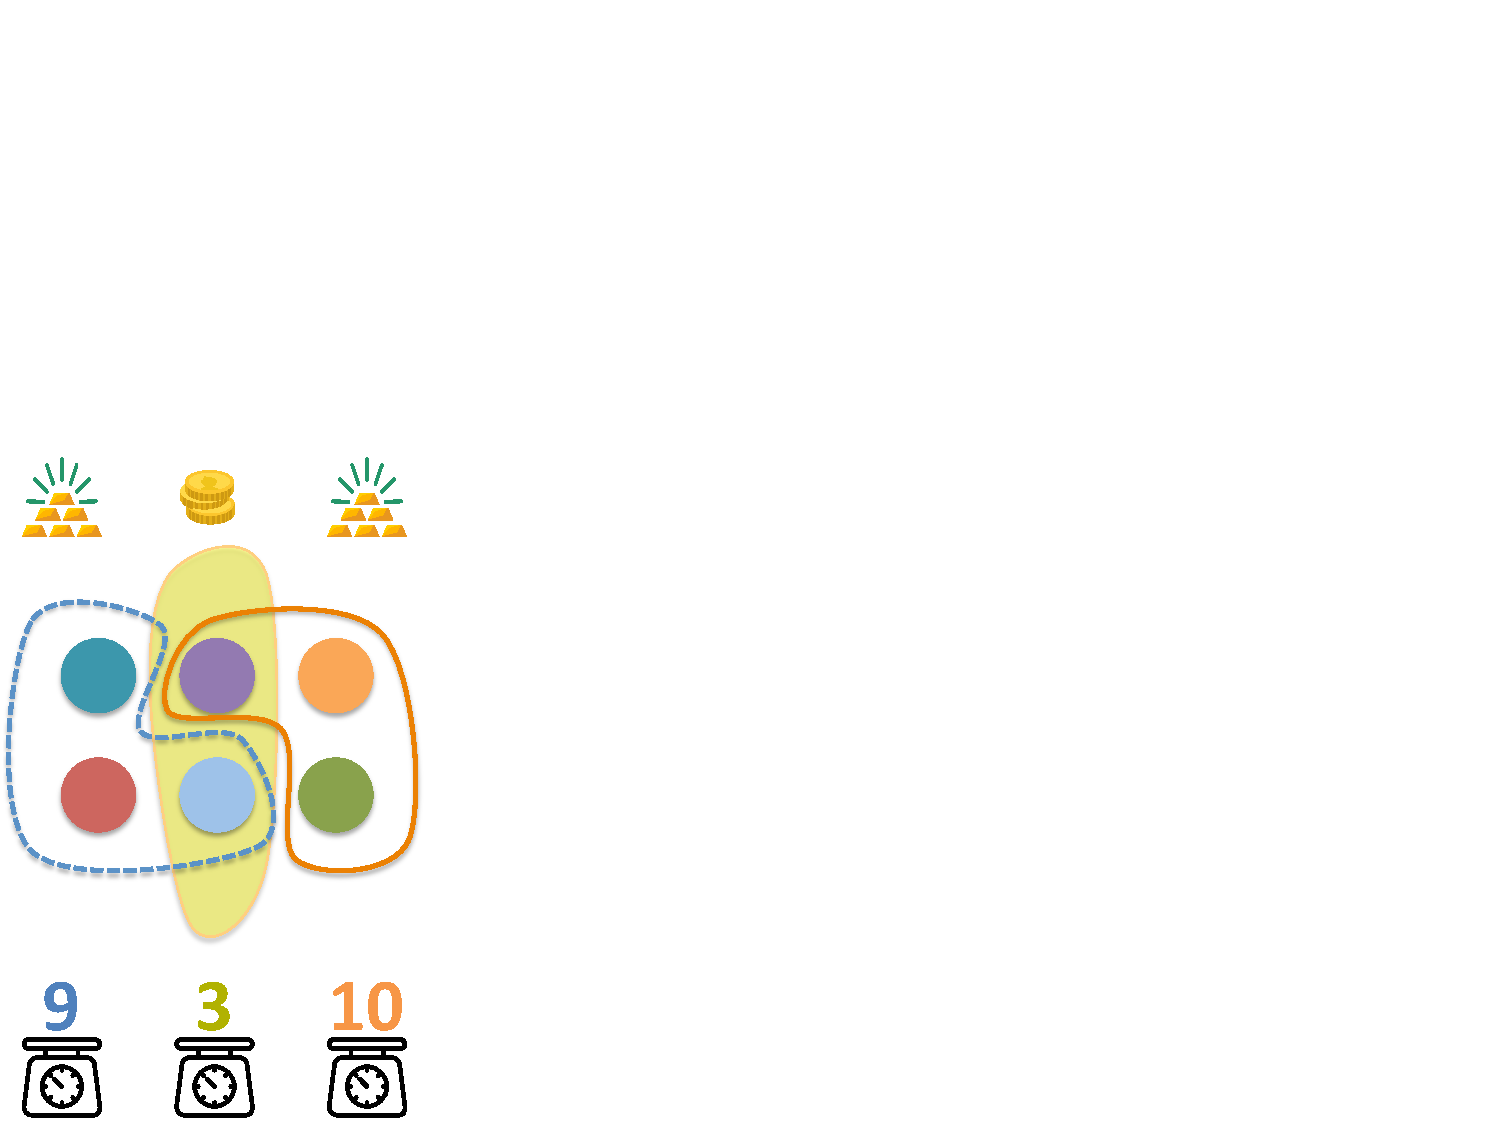
\includegraphics[width=\columnwidth]{value.pdf}\vfill}% 
\end{overlayarea}%
\end{minipage}%
\begin{minipage}{0.70\textwidth} 
\begin{itemize}
\item<1-> Elements with frequency $1$ should be covered first
\item<2-> Extend idea to \textbf{``infrequent''} elements
\item<3-> Assign a value to each element
  	$$ \text{value(element)} = \cfrac{1}{\text{frequency-1}}$$
\item<4-> Assign value to each set
	$$ \text{value(set)} = \sum \text{value(element)}$$
\item<5> Choose a set with \textbf{small weight} and \textbf{large value!}
\end{itemize}
\end{minipage}
\end{frame}

\begin{frame}
\frametitle{Heuristics, General Framework}
\begin{minipage}{0.30\textwidth}
\begin{overlayarea}{\textwidth}{0.5\textheight}
\only<1-2>{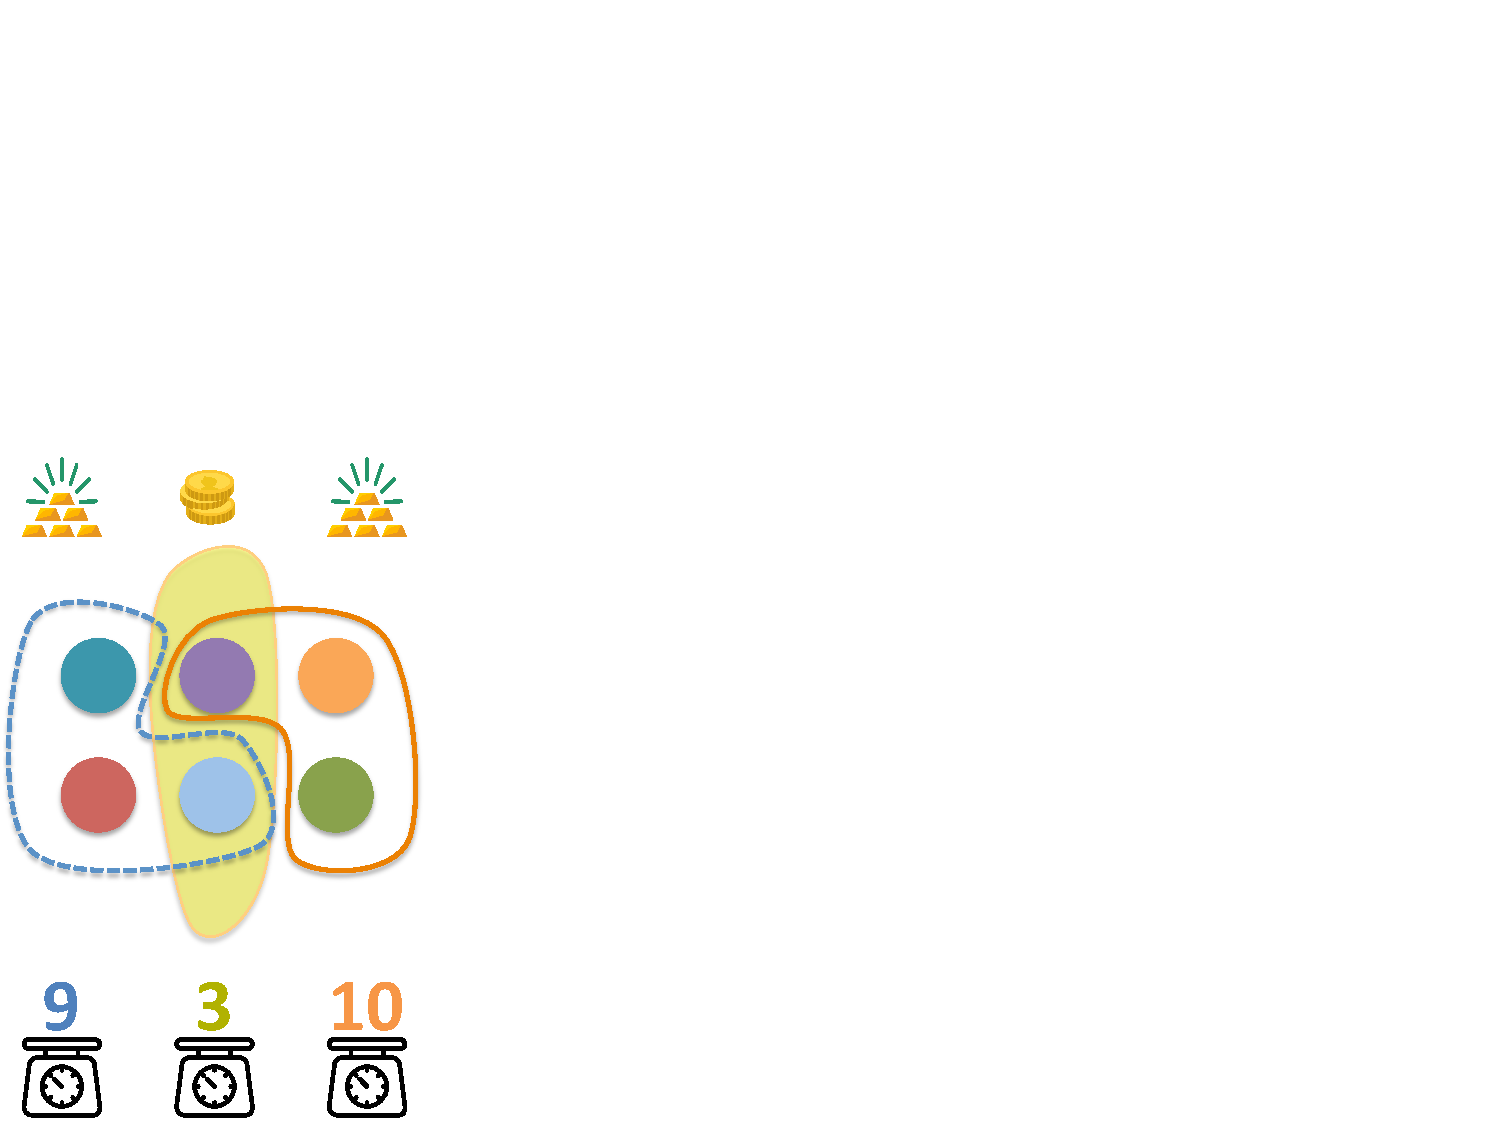
\includegraphics[width=\columnwidth]{value.pdf}\vfill}% 
\end{overlayarea}%
\end{minipage}%
\begin{minipage}{0.70\textwidth} 
\begin{itemize}
\item<1-> New Greedy Choice 
$$ best\_set = \arg \min_{j} \cfrac{w_j}{v_j} = \arg \min_{j} \cfrac{w_j}{\sum \text{value}(e_i)} $$
\item<2> Regular Greedy is a Special Case
 $$ \text{if value}(e_i) = 1 \rightarrow \cfrac{w_j}{\sum\text{value}(e_i)} = \cfrac{w_j}{|\hat{S}_j|}$$
\end{itemize}
\end{minipage}
\end{frame}

\begin{frame}
\frametitle{Another Heuristic Valuation..}
Dig Deeper, Extract more Information \inlinegraphics{excavators.eps}
$$ \text{value}(e_i) = \cfrac{\sum_{S_j: e_i \in S_j} \text{average\_weight}(S_j)}{\text{frequency}(e_i)-1}$$
An element is valuable if it is contained in ``expensive'' sets.

[\textbf{Intuition}] Choose a ``\textbf{cheap}'' set that contains elements that are ``\textbf{expensive in the market}''.
\end{frame}

\begin{frame}
\frametitle{Value Functions Tested}
\begin{minipage}{0.50\textwidth}
\begin{itemize}
\item Greedy: $v(e_i) = 1$
\item H 1: $v(e_i) = \cfrac{1}{f_i -1}$
\item H 2: $v(e_i) = 1+\cfrac{1}{f_i -1}$
\item H 3: $v(e_i) = exp(-f_i)$
\item H 4: $v(e_i) = \cfrac{|\hat{S}_j|}{f_i -1}$
\item H 7: $v(e_i) = \cfrac{1}{(f_i -1)^2}$

\end{itemize}
\end{minipage}%
\begin{minipage}{0.50\textwidth}
\begin{itemize}
\item H 8: $v(e_i) = \cfrac{1}{(f_i -1)^3}$
\item H 9: $v(e_i) = \cfrac{1}{\sqrt{f_i -1}}$
\item H 10: $v(e_i) = \cfrac{\sum w_j/|\hat{S}_j|}{f_i -1}$
\item H 11: $v(e_i) = c + \cfrac{\sum w_j/|\hat{S}_j|}{f_i -1}$
\end{itemize}
\end{minipage}
\end{frame}

\begin{frame}
\frametitle{Data Sets}
\end{frame}

\begin{frame}
\frametitle{Experimental Results}
\end{frame}

\begin{frame}
\frametitle{References}
\end{frame}

\end{document}
